\documentclass[10pt]{beamer}
\usepackage{beamerthemesplit}
\usetheme{madrid}
%\usecolortheme{crane}

\usepackage[T2A]{fontenc}
%\usepackage[cp1251]{inputenc} %for Windows
\usepackage[utf8]{inputenc}


%\documentclass[a4paper, 1wpt]{amsart}
\usepackage[english]{babel}
\usepackage{graphics}
\usepackage{amsfonts, amssymb, amscd, amsmath}
\usepackage{latexsym}
\usepackage[matrix,arrow,curve]{xy}
\usepackage{mathabx}%,mathtools}
\usepackage{color}
\usepackage{pbox}
\usepackage{tikz}
\usepackage{array}
%\usetikzlibrary{matrix,decorations.pathreplacing,positioning}
%\usepackage{scalerel}
\usepackage{hyperref}

\usepackage{parskip}
\usepackage{array}
\usepackage{epigraph}
\usepackage{animate}
\usepackage{stackrel}

%\DeclareSymbolFont{cyrillic}{T2A}{cmr}{m}{n}
%\DeclareMathSymbol{\Tse}{\mathalpha}{cyrillic}{214}


\newcolumntype{M}[1]{>{\centering\arraybackslash}m{#1}}

%\renewcommand{\contentsname}{GGGGGGGGGGGGG}

\definecolor{emph}{RGB}{200,90,0}

\newcolumntype{P}[1]{>{\centering\arraybackslash}p{#1}}

\DeclareMathOperator{\Cone}{Cone}
\DeclareMathOperator{\pt}{pt}
\DeclareMathOperator{\Ker}{Ker}
\DeclareMathOperator{\id}{id}
\DeclareMathOperator{\codim}{codim}
\DeclareMathOperator{\sgn}{sgn}
\DeclareMathOperator{\Imm}{Im}
\DeclareMathOperator{\im}{Im}
\DeclareMathOperator{\supp}{supp}
\DeclareMathOperator{\const}{const}
\DeclareMathOperator{\Hom}{Hom}
\DeclareMathOperator{\rk}{rk}
\DeclareMathOperator{\diag}{diag}
\DeclareMathOperator{\conv}{conv}
\DeclareMathOperator{\tr}{tr}
\DeclareMathOperator{\re}{Re}
\DeclareMathOperator{\PH}{PH}
\DeclareMathOperator{\EMST}{EMST}
\DeclareMathOperator{\LMST}{LMST}
\DeclareMathOperator{\Hilb}{P}

\DeclareMathOperator{\Sym}{Sym}

\DeclareMathOperator{\nc}{nc}


\DeclareMathOperator{\dist}{dist}
\DeclareMathOperator{\grad}{grad}

\newcommand{\ko}{\Bbbk}
\newcommand{\Fo}{\mathbb{F}}
\newcommand{\Zo}{\mathbb{Z}}
\newcommand{\Ro}{\mathbb{R}}
\newcommand{\Rg}{\mathbb{R}_{\geqslant 0}}
\newcommand{\Co}{\mathbb{C}}
\newcommand{\Qo}{\mathbb{Q}}
\newcommand{\Noo}{\mathbb{N}}
\newcommand{\Zt}{\Zo_2}
\newcommand{\Eo}{\mathbb{E}}

\newcommand{\br}{\widetilde{\beta}}
\newcommand{\eqd}{\stackrel{\text{\tiny def}}{=}}
\newcommand{\toiso}{\stackrel{\cong}{\to}}

\newcommand{\wh}[1]{{\widehat{#1}}}
\newcommand{\ca}[1]{\mathcal{#1}}

\newcommand{\Ch}{\check{C}}

\newcommand{\Hr}{\widetilde{H}}
\newcommand{\dd}{\partial}
\newcommand{\Ca}{\mathcal{C}}
\newcommand{\F}{\mathcal{F}}


\newcommand{\RP}{\mathbb{R}P}
\newcommand{\CP}{\mathbb{C}P}


\title[Topology intro]{Topological data analysis \\ Lecture 2}
\author[Anton Ayzenberg]{ Anton Ayzenberg }% \\  \texttt{ayzenberga@gmail.com}}
\date[FCS-YDS'24]{Spring 2024 \\ Faculty of Computer Science / Yandex Data School}
\institute[ATA \& Noeon Research]{ATA Lab, FCS NRU HSE \\ Noeon Research}

\begin{document}

\maketitle



\begin{frame}{Counting cycles in a graph}

\begin{center}
\includegraphics[scale=0.12]{pictures/graphcycles.pdf}
\end{center}

\end{frame}

\begin{frame}{Vector space of cycles}

\begin{itemize}
  \item ``The number of cycles'' is the number of \textcolor{red}{basic cycles}.
  \item Basic cycles = any collection of cycles, from which all other cycles are expressed uniquely as sums over $\Zt$ (field with 2 elements).
  \item In other words, let $Z_1(\Gamma;\Zt)$ denote the vector space (over $\Zt$) of all algebraical cycles.
  \item Algebraical cycle = collection of edges, such that even number of edges meet in each vertex.
  \item Then the number of cycles = $\dim Z_1(\Gamma;\Zt)$.
\end{itemize}

\end{frame}

\begin{frame}{More abstract characterization}

\begin{itemize}
  \item $C_1(\Gamma;\Zt)=\Zt\langle\mbox{edges of }\Gamma\rangle$;
  \item $C_0(\Gamma;\Zt)=\Zt\langle\mbox{vertices of }\Gamma\rangle$;
  \item $\dd_1\colon C_1(\Gamma;\Zt)\to C_0(\Gamma;\Zt)$.
  \item where $\dd(\{v_1,v_2\})=v_1\oplus v_2$.
  \item Then $\sigma\in C_1(\Gamma;\Zt)$ is a cycle iff $\dd_1(\sigma)=0$.
  \item Therefore $Z_1(\Gamma;\Zt)=\Ker\dd_1$.
  \item We define $H_1(\Gamma;\Zt)=Z_1(\Gamma;\Zt)$ and \textbf{the first Betti number} $\beta_1(\Gamma)=\dim H_1(\Gamma;\Zt)$.
\end{itemize}

\end{frame}

\begin{frame}{First homology, graph case}

\begin{itemize}
  \item We define $H_1(\Gamma;\Zt)=Z_1(\Gamma;\Zt)$ and \textbf{the first Betti number} $\beta_1(\Gamma)=\dim H_1(\Gamma;\Zt)$.
  \item This number counts cycles in a graph.
  \item In graph theory it is called \textbf{circuit rank}.
\end{itemize}

\begin{block}{Remark}
The matrix of $\dd_1\colon C_1(\Gamma;\Zt)\to C_0(\Gamma;\Zt)$ is the incidence matrix of a graph
\[
D_1=\begin{array}{c|ccc}
& \cdots  & e & \cdots \\
\hline
\vdots &  & \vdots &  \\
v & \cdots & \varepsilon_{v,e} & \cdots  \\
\vdots &  & \vdots &
\end{array}
\]
\end{block}

We have $\beta_1(\Gamma)=\dim\Ker\dd_1=\#\mbox{edges}-\rk D_1$. This can be computed by \textcolor{red}{Gauss algorithm}.

\end{frame}

\begin{frame}{Graph homology from other invariants}

We have $\beta_1(\Gamma)=\dim\Ker\dd_1=\#\mbox{edges}-\rk D_1$.

\textbf{Exercise:} $\dim \Imm\dd_1 (=\rk D_1)=\#\mbox{vertices}-\#\mbox{con.components}$.

\begin{block}{Corollary}
\[
\beta_1(\Gamma)=\#\mbox{edges}-\#\mbox{vertices}+\#\mbox{con.components}.
\]
\end{block}

Do you recognize the number \textcolor{red}{$\#\mbox{vertices}-\#\mbox{con.components}$}? \pause

It follows that $\beta_1(\Gamma)$ equals the number of edges remaining after removal of (any) spanning forest.
\end{frame}

\begin{frame}{First homology of a simp. complex}
\pause

\begin{center}
\includegraphics[scale=0.3]{pictures/cycles1.pdf}
\end{center}

\end{frame}

\begin{frame}{First homology of a simp. complex}

\begin{itemize}
  \item Homology = ``cycles, which are not boundaries''.
  \item ``Number of holes = number of cycles - number of boundaries''.\pause
  \item $Z_1(K;\Zt)=\Ker\dd_1\colon C_1(K;\Zt)\to C_0(K;\Zt)$ the space of 1-cycles.
  \item $B_1(K;\Zt)\subset Z_1(K;\Zt)$ : the space generated by boundaries of triangles.\pause
  \item $B_1(K;\Zt)=\Imm\dd_2\colon C_2(K;\Zt)\to C_1(K;\Zt)$ where
  \item $\dd_2(\{v_1,v_2,v_3\})=\{v_1,v_2\}\oplus\{v_2,v_3\}\oplus \{v_3,v_1\}$ is the boundary of a triangle.
  \item $H_1(K;\Zt)=Z_1(K;\Zt)/B_1(K;\Zt)$ (the quotient vector space).
\end{itemize}

\end{frame}

\begin{frame}{Betti number}

\begin{itemize}
  \item $H_1(K;\Zt)=Z_1(K;\Zt)/B_1(K;\Zt)$.
  \item $\beta_1(K)=\dim H_1(K;\Zt)$.
  \item This number counts ``the number of 1-dim. holes in $K$''.
\end{itemize}
\pause

The definition is consistent with graphs. For graphs we have no triangles, hence $C_2(\Gamma;\Zt)=0$ hence $B_1(\Gamma;\Zt)=0$ hence $H_1(\Gamma;\Zt)=Z_1(\Gamma;\Zt)$.
\pause

To compute $\beta_1$, one needs $\rk D_1$ (the incidence matrix between edges and vertices) and $\rk D_2$, where $D_2$ is \textcolor{red}{``the incidence matrix''} between triangles and edges.

\textbf{Exercise:} $\beta_1(K)=\#\mbox{edges}-\rk D_1-\rk D_2$.
\end{frame}


\begin{frame}{General definitions}

Let $K$ be a simplicial complex, and $\ko$ be a field.

\begin{itemize}
  \item $C_j(K;\ko)$ : the $\ko$-vector space spanned freely by $j$-dimensional simplices of $K$.
  \item $C_j(K;\ko)$ is called the space of $j$-dim simplicial chains of $K$.
  \item $\dd_j\colon C_j(K;\ko)\to C_{j-1}(K;\ko)$ : $j$-th boundary operator, also called simplicial differential.
  \item $\dd_j(\{v_0,v_1,\ldots,v_j\})=\{v_1,\ldots,v_j\}-\{v_0,v_2,\ldots,v_j\}+\cdots+(-1)^j\{v_0,v_1,\ldots,v_{j-1}\}$.
\end{itemize}

\textbf{Exercise:} Prove that $\dd_{j}\circ\dd_{j+1}=0$. \textcolor{red}{``There is no boundary of a boundary''}.

\end{frame}

\begin{frame}{Boundaries}

\begin{itemize}
  \item $\dd_j(\{v_0,v_1,\ldots,v_j\})=\{v_1,\ldots,v_j\}-\{v_0,v_2,\ldots,v_j\}+\cdots+(-1)^j\{v_0,v_1,\ldots,v_{j-1}\}$.
  \item ``There is no boundary of a boundary''.
\end{itemize}

\begin{center}
\includegraphics[scale=0.3]{pictures/boundaries.pdf}
\end{center}

\end{frame}

\begin{frame}{General definitions}
\begin{itemize}
  \item $C_j(K;\ko)$ : the vector space of $j$-dim chains.
  \item $\dd_j\colon C_j(K;\ko)\to C_{j-1}(K;\ko)$ : $j$-th boundary operator.
  \item $Z_j(K;\ko)=\Ker \dd_j$ : the vector space of $j$-dim cycles.
  \item $B_j(K;\ko)=\Imm \dd_{j+1}$ : the vector space of $j$-dim boundaries.\pause
  \item Exercise implies $B_j(K;\ko)\subseteq Z_j(K;\ko)$.
\end{itemize}

\begin{block}{Definition}
The quotient space $H_j(K;\ko)=Z_j(K;\ko)/B_j(K;\ko)$ is called the \textbf{$j$-th simplicial homology module} of $K$.
\end{block}

\end{frame}

\begin{frame}{Homology}

\[
\mbox{Homology: }
H_j(K;\ko)=Z_j(K;\ko)/B_j(K;\ko)
\]

$j$-th Betti number
\[
\beta_j(K)=\dim H_j(K;\ko) = \dim Z_j(K;\ko) - \dim B_j(K;\ko).
\]

\begin{itemize}
  \item $\beta_j(K)$ counts the number of $j$-dim holes in $K$.\pause
  \item \textbf{Exercise 1:} $\beta_0(K)$ equals the number of connected components of $K$.\pause
  \item \textbf{Exercise 2:} $\beta_j(K)=\# j\mbox{-dim simplices}-\rk D_j - \rk D_{j+1}$, where $D_j$ is the matrix of $\dd_j$. This is the incidence matrix between $j$-dim simplices and $(j-1)$-dim simplices.
\end{itemize}

Therefore we need $C_{j-1}(K;\ko)$, $C_{j}(K;\ko)$, $C_{j+1}(K;\ko)$, $\dd_j$, and $\dd_{j+1}$ to compute $\beta_j(K)$.

\end{frame}

\begin{frame}{Old but instructive meme}

\begin{center}
\includegraphics[scale=0.2]{pictures/meme.jpg}
\end{center}

\end{frame}

\begin{frame}{Homology is an invariant of homotopy equivalence}

\begin{itemize}
  \item $K$ : a simplicial complex;
  \item $|K|$ : its geometrical realization in some $\Ro^d$ (a picture).
\end{itemize}

\begin{block}{Fact:}
\begin{enumerate}
  \item Homeomorphism. If $|K|\cong |L|$ then $H_j(K;\ko)\cong H_j(L;\ko)$.
  \item Homotopy equivalence. If $|K|\simeq |L|$ then $H_j(K;\ko)\cong H_j(L;\ko)$.
\end{enumerate}
\end{block}

We will not prove it here, but we will be using this fact.

\end{frame}




\begin{frame}{Examples and calculations}

\textcolor{red}{Example 0:} if $\pt$ is the one-point space, then $\beta_0(\pt)=1$ and $\beta_j(\pt)=0$ for $j>0$.

\begin{block}{Homology are invariants}
If $X\simeq Y$ then $\beta_j(X)= \beta_j(Y)$. Homology do not depend on triangulations of $X$ and $Y$.
\end{block}
\pause

\textcolor{red}{Example 1:} $D^n=\{x\in \Ro^n\mid \|x\|\leqslant 1\}$ is called an $n$-disk. Exercise: $D^n\simeq \pt$. So far, disk does not have interesting homology.
\pause

\textcolor{red}{Example 2:} $S^{n-1}=\{x\in \Ro^n\mid \|x\|=1\}$. We have $S^{n-1}=\dd D^n$. Exercise: prove that $\beta_j(S^{n-1})=1$ if $j=0$ or $n-1$, and all other Betti numbers are zero.

\textcolor{blue}{Hint:} Represent $S^{n-1}$ as the boundary $\dd\Delta^n$ of a simplex. This is a simplicial complex on $n+1$ vertices whose simplices are $2^{[n+1]}\setminus[n+1]$. Understand the relation between chain spaces of $\dd\Delta^n$ and that of $\Delta^n$.

\end{frame}


\begin{frame}{Examples and calculations}

\begin{center}
\includegraphics[scale = 0.15]{pictures/KleinBottle.png}
\end{center}

\textbf{Exercise:} Triangulate Klein bottle somehow, and compute its homology with coefficients in $\Zt$, $\Zo_3$, and $\Qo$.

\textbf{Exercise:} Find $H_j(K;\Zt)$, where $K$ is the 2-skeleton of 4-dim simplex (simp.comp. on $[5]=\{1,2,3,4,5\}$, which consists of all subsets of cardinality $\leqslant 3$).

\textbf{Exercise:} Consider the simp.comp. $U_3$, whose vertex set is the set of all nonzero vectors of $\Zt^3$ (7 vertices in total), and simplices are exactly those subsets, which correspond to linearly independent collections of vectors. Compute $\beta_j(U_3;\Zt)$.
\end{frame}

\begin{frame}{K\"{u}nneth formula}

Consider the generating function of Betti numbers
\[
\Hilb(X;t)=\sum_j \beta_j(X)t^j,
\]
called \textcolor{red}{Poincar\'{e} polynomials} (or Hilbert--Poincar\'{e} polynomials) of a space $X$.\pause

\textbf{Exercise:} $\Hilb(X\sqcup Y;t)=\Hilb(X;t)+\Hilb(Y;t)$.\pause

\textcolor{red}{Example:} $\Hilb(S^n;t)=1+t^n$.\pause

\begin{block}{K\"{u}nneth theorem}
\[
\Hilb(X\times Y;t)=\Hilb(X;t)\cdot \Hilb(Y;t)
\]
\end{block}
\pause

\textcolor{red}{Example:} $T^n=S^1\times\cdots\times S^1$ is called the $n$-dimensional torus. We have $\Hilb(T^n;t)=(1+t)^n$, so $\beta_j(T^n)={n\choose j}$.
\end{frame}

\begin{frame}{Functoriality}

\begin{itemize}
  \item Let $L\subset K$ be \textcolor{blue}{a simplicial subcomplex}:
  \item which means every simplex of $L$ is also a simplex of $K$.\pause
  \item Then every $j$-cycle in $L$ is also a $j$-cycle in $K$ that is $Z_j(L;\ko)\subset Z_j(K;\ko)$.
  \item And every $j$-boundary in $L$ is also a $j$-boundary in $K$ that is $B_j(L;\ko)\subset B_j(K;\ko)$.\pause
  \item We have a linear map
  \[
  \xymatrix{
  H_j(L;\ko) \ar@{=}[d] \ar@{->}[r]^{f_{L\subset K}} & H_j(K;\ko) \ar@{=}[d]  \\
  Z_j(L;\ko)/B_j(L;\ko) \ar@{->}[r] & Z_j(K;\ko)/B_j(K;\ko)
  }
  \]
  called \textbf{the induced map of inclusion} $L\hookrightarrow K$.
\end{itemize}

\end{frame}





\begin{frame}{Sources}

\begin{thebibliography}{12}

\bibitem{EH} H.\,Edelsbrunner, J.\,L.\,Harer, Computational Topology: An Introduction, 2010.

\bibitem{Ghr} R.\,Ghrist, Elementary applied topology, available \href{https://www2.math.upenn.edu/~ghrist/notes.html}{online}.

\bibitem{Hatcher} A.\,Hatcher, Algebraic topology, 2002.

\bibitem{Zom} A.\,J.\,Zomorodian, Topology for computing, 2005.

\end{thebibliography}

\end{frame}



%\begin{frame}{Technical slide}
%\href{https://colab.research.google.com/drive/146yQdZBsPGfYZwi1AGKJwSE5wjRwPnc1?usp=sharing}{Colab}
%
%\href{https://play.unity.com/mg/other/builds-4z-1}{Unity}
%
%\begin{center}
%\animategraphics[controls,scale=0.25]{5}{pictures/Simplify/Simplify_}{0}{1}
%\end{center}
%\end{frame}


\end{document}
